
\documentclass[letterpaper,12pt]{article}
\usepackage{tabularx} % extra features for tabular environment
\usepackage{amsmath}  % improve math presentation
\usepackage{float}
\usepackage{pdfpages}

\usepackage{multicol}
\usepackage{graphicx} % takes care of graphic including machinery
\graphicspath{ {./figures/} }
%\usepackage[margin=1in,letterpaper]{geometry} % decreases margins
%\usepackage{cite} % takes care of citations
\usepackage[final]{hyperref} % adds hyper links inside the generated pdf file
\hypersetup{
	colorlinks=true,       % false: boxed links; true: colored links
	linkcolor=blue,        % color of internal links
	citecolor=blue,        % color of links to bibliography
	filecolor=magenta,     % color of file links
	urlcolor =blue         
}
\usepackage[margin = 1in,headsep=0.5cm,headheight=2cm,letterpaper]{geometry} 

\usepackage{fancyhdr}
\pagestyle{fancy}
%\cfoot{center of the footer!}
\renewcommand{\headrulewidth}{0.1pt}



\begin{document}
\thispagestyle{empty}

\title{Fall 2022 EE301  \protect\\ Homework 1}
\author{Ahmet Akman 2442366 \protect\\ Hasan Oğuzhan Gök 2443083 }
\date{\today}
\maketitle
\tableofcontents
%\begin{abstract}
%abstract
%\end{abstract}
\section{Question 1 Solution}
Input/output relation: \(y_1(t)= x(t)cos(2 \pi f_0 t) \)
\\ Properties:

\begin{itemize}
    \item \textbf{Memory:} 
    \item \textbf{Linearity:}
    \item \textbf{Causality:}
    \item \textbf{Time-Invariance:}
    \item \textbf{Stability:}
\end{itemize}
Input/output relation: \(y_2(t)= c_1 x(t) + c_2 x^2(t) \)
\\ Properties:
\begin{itemize}
    \item \textbf{Memory:} 
    \item \textbf{Linearity:}
    \item \textbf{Causality:}
    \item \textbf{Time-Invariance:}
    \item \textbf{Stability:}
\end{itemize}

Input/output relation: \(y_3(t)= x(t)+4 \)
\\ Properties:
\begin{itemize}
    \item \textbf{Memory:} 
    \item \textbf{Linearity:}
    \item \textbf{Causality:}
    \item \textbf{Time-Invariance:}
    \item \textbf{Stability:}
\end{itemize}

Input/output relation: \(y_4(t)= x(t/3) \)
\\ Properties:
\begin{itemize}
    \item \textbf{Memory:} 
    \item \textbf{Linearity:}
    \item \textbf{Causality:}
    \item \textbf{Time-Invariance:}
    \item \textbf{Stability:}
\end{itemize}

Input/output relation: \(y_5(t)= t x(t+5) \)
\\ Properties:


\begin{itemize}
    \item \textbf{Memory:} 
    \item \textbf{Linearity:}
    \item \textbf{Causality:}
    \item \textbf{Time-Invariance:}
    \item \textbf{Stability:}
\end{itemize}

Input/output relation: \(y_6(t)= u(x(t)) \)
\\ Properties:
\begin{itemize}
    \item \textbf{Memory:} 
    \item \textbf{Linearity:}
    \item \textbf{Causality:}
    \item \textbf{Time-Invariance:}
    \item \textbf{Stability:}
\end{itemize}



\section{Question 2 Solution}
\subsection{a)}

\subsection{b)}
\section{Question 3 Solution}
\subsection{a)}
\subsection{b)}
\subsection{c)}
\subsection{d)}
\subsection{e)}
\subsection{f)}

\section{Question 4 Solution}
\subsection{a)}
\subsection{b)}
\subsection{c)}

\subsubsection{i)}

\subsubsection{ii)}
\section{Question 5 Solution}
\subsection{a)}
In part 5, we convolved the input signal \(x[n] = sin(\frac{2\pi n}{7} )\) and impulse response \(h[n] = u[n] - u[n-L]\) to find output signal \(y[n]\) in MATLAB.
\subsubsection{i)}
In this part N(signal length) was equal to 20. Then following signal was plotted.
\begin{figure}[H]
    \centering
    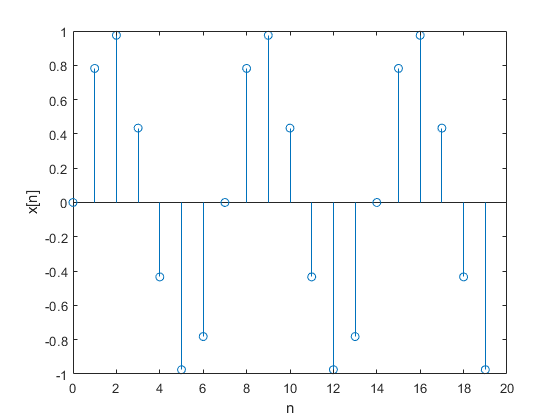
\includegraphics[width = 0.75\textwidth]{i.png}
    \caption{Signal x[n]}
    \end{figure} 
    
\subsubsection{ii)}
Impulse response \(h[n]\) was created with amplitude 1 and pulse duration L. L was equal to 14 in this example.
\begin{figure}[H]
    \centering
    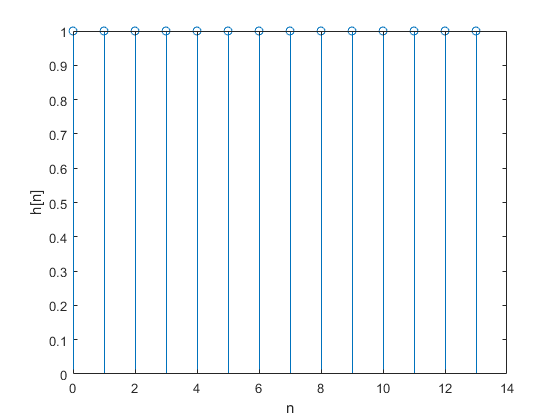
\includegraphics[width = 0.75\textwidth]{i2.png}
    \caption{Impulse Response}
    \end{figure} 
    
\subsubsection{iii)}
In this part we implemented convolution operation. Since our signals are not infinity we used zero padding to be able to compute convolution. Then we obtained \(y[n]\) using for loop. Since zero padding leads to mistake on last a few values, we only plotted correct ones. Following plot shows the output of convolution operation with padding.
\begin{figure}[H]
    \centering
    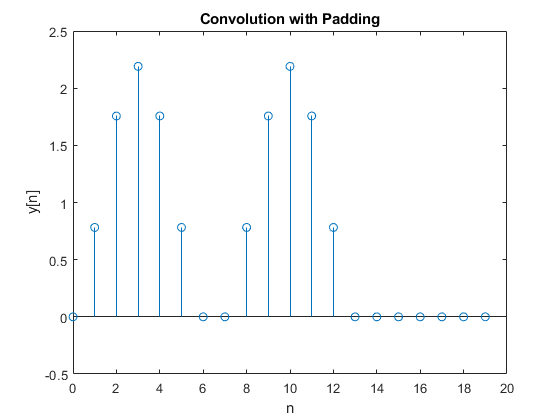
\includegraphics[width = 0.75\textwidth]{convwithpadding.png}
    \caption{Convolution with Padding}
    \end{figure} 
    
\subsubsection{iv)}
Convolution operation executed in last part can be done by conv method in MATLAB. Following graph shows the convolution results. 
\begin{figure}[H]
    \centering
    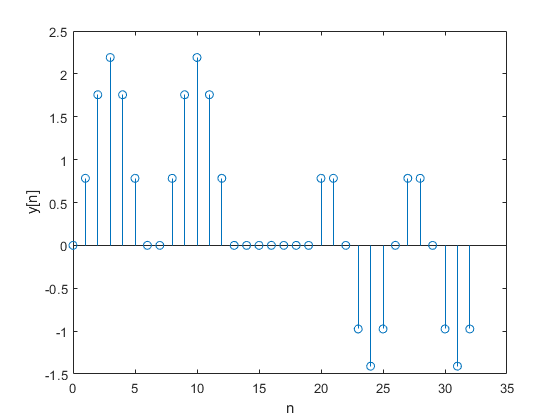
\includegraphics[width = 0.75\textwidth]{i4.png}
    \caption{Convolution Operation Using conv Method}
    \end{figure} 
    As indicated in figures in section iii and iv , the convolution method in MATLAB results in more acquarete results. Due to the zero padding method in part iii, results after n>N are nor correct.


\subsection{b)}
To observe pulse duration length(L) effect on output signal, random signal input convolved with \(h[n]\) by changing L in the \(h[n] = u[n] - u[n-L]\). L was chossen to be 2 , 15 and 25.
Following graph shows the random signal \(x[n]\).
\begin{figure}[H]
    \centering
    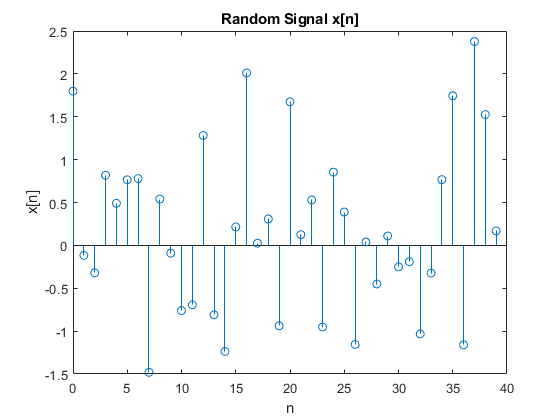
\includegraphics[width = 0.75\textwidth]{b_signal.png}
    \caption{Random Signal}
    \end{figure} 


The convolution result \(y[n] = x[n] * h[n]\) with L = 2 is shown in following figure.
\begin{figure}[H]
    \centering
    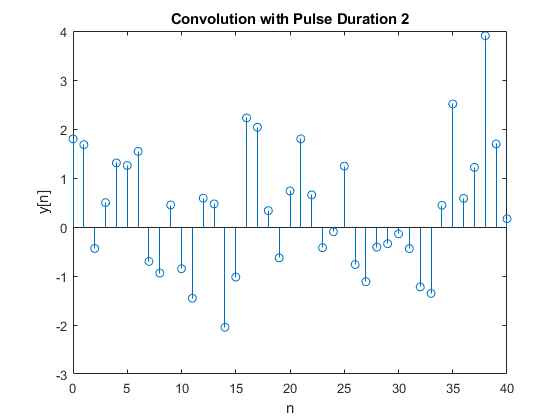
\includegraphics[width = 0.75\textwidth]{b_duration2.png}
    \caption{Convolution Result with L=2}
    \end{figure} 


    The convolution result \(y[n] = x[n] * h[n]\) with L = 15 is shown in following figure.
    \begin{figure}[H]
        \centering
        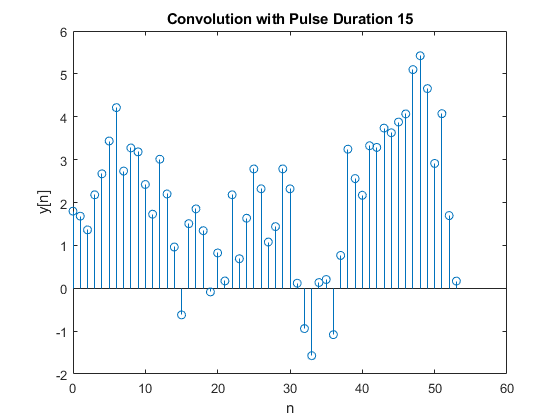
\includegraphics[width = 0.75\textwidth]{b_duration15.png}
        \caption{Convolution Result with L=15}
        \end{figure} 

        
        The convolution result \(y[n] = x[n] * h[n]\) with L = 25 is shown in following figure. 
        \begin{figure}[H]
            \centering
            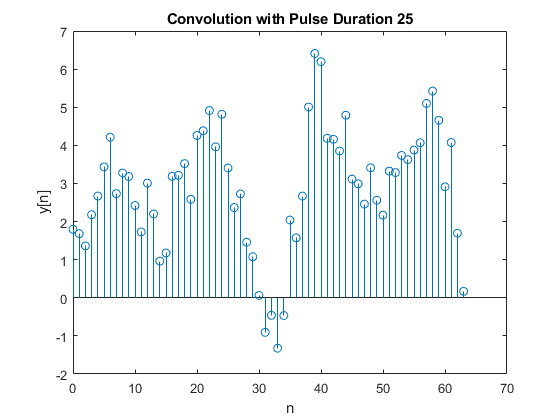
\includegraphics[width = 0.75\textwidth]{b_duration25.png}
            \caption{Convolution Result with L=25}
            \end{figure} 



As shown in al figures, the smoothness of graph increases as L increases. Although it gets smoother, these systems called "averaging filter" ,may lead to some loses. This filter can be used to observe a signal's trend and obtain meaningfull data.




\end{document}

%%%%%%%%%%%%%%%%%%%%%%   EXAMPLE TABLE   %%%%%%%%%%%%%%%%%%%%%%%%%%%%%%%%
\begin{table}[H]
\begin{center}
    \caption{Resistance reading by color code convention.}
    \vspace{2mm}
    \begin{tabular}{||c | c | c||} 
        \hline
        Color Order & Value & Tolerance \\ [0.5ex] 
        \hline\hline
        Brown / Black / Red / Gold & 1k\( \Omega \) & \( \% \) 5  \\ 
        \hline
        Yellow / Violet / Red / Gold & 4.7k\( \Omega \) & \( \% \) 5   \\
        \hline
        Brown / Grey / Orange / Gold & 18k\( \Omega \) & \( \% \) 5  \\ [1ex] 
        \hline
    \end{tabular}
\end{center}
\end{table}


%%%%%%%%%%%%%%%%%%%%%%   EXAMPLE IMAGE   %%%%%%%%%%%%%%%%%%%%%%%%%%%%%%%%
\begin{figure}[H]
\centering
\includegraphics[width = 0.75\textwidth]{5.png}
\caption{Circuit schematic for the step 5}
\end{figure} 

%%%%%%%%%%%%%%%%%%%%%%   EXAMPLE IMAGE FROM PDF   %%%%%%%%%%%%%%%%%%%%%%%%%%%%%%%%
\begin{figure}[H] \centering{
	\includegraphics[scale=0.25]{2a_plot.pdf}}
	\caption{Experiment 2}
\end{figure}
